\documentclass[a4paper]{article}
\usepackage[font=small,labelfont=bf]{caption}
\usepackage[T1]{fontenc}
\usepackage[utf8]{inputenc}
\usepackage[english]{babel}
\usepackage{url} % per scrivere gli indirizzi url
\usepackage{booktabs}
\usepackage{graphicx}
\usepackage[left=1.5cm,bottom=1.5cm,right=1cm,top=2.5cm]{geometry}
\usepackage{frontespizio}
\usepackage{wrapfig}
\usepackage{xcolor}
\usepackage{color}
\usepackage{siunitx}  
\usepackage{hyperref}
\usepackage{listings}
\usepackage{framed} 
\usepackage{parskip} %risolve i dannati indent.
\usepackage{fancyvrb}
\usepackage{graphicx}

\definecolor{comment}{RGB}{237, 141, 33}
\definecolor{backy}{RGB}{ 255, 253, 183 }
\definecolor{back}{RGB}{ 30,30,30 }
\definecolor{shadecolor}{RGB}{ 30,30,30 }
\lstset{
%rulecolor=\color{white},
numbers=left,
numberstyle=\color{black},
%backgroundcolor=\color{back},   
frame=single,
showspaces=false,
basicstyle=\ttfamily,%\color{white},
showstringspaces=false,
keywordstyle=\color{purple},       % keyword style
commentstyle=\color{comment},    % comment style
stringstyle=\color{blue}    % string literal style
}

\begin{document}
\begin{center}
\begin{Large}
Università degli studi di Bergamo
\end{Large}
\end{center}
\begin{center}
\begin{Large}
Facoltà di Ingegneria
\end{Large}
\end{center}
\begin{center}
\begin{Large}
Corso di Laurea Magistrale in Ingegneria Informatica
\end{Large}
\end{center}

\vspace{1\baselineskip}

\begin{center}

\includegraphics[scale=0.6]{UniBG.png}
\end{center}

\vspace{1\baselineskip}

\begin{center}
\begin{Large}
Corso di Linguaggi formali e compilatori
\end{Large}
\end{center}
\begin{center}
\begin{Large}
Anno accademico 2018/2019
\end{Large}
\end{center}

\vspace{3\baselineskip}

\begin{center}
\begin{Huge}
G8 practical manual
\end{Huge}
\end{center}
\begin{center}
\begin{Huge}
From the basics to a complete example
\end{Huge}
\end{center}

\vspace{3\baselineskip}

\begin{Large}
\begin{center}
Stefano Villa, Matricola 1055820\\
Matteo Zambelli, Matricola 1055560
\end{center}
\end{Large}

\newpage
\tableofcontents
\newpage

\section{Introduction}

HTML5 element <canvas> gives you an easy and powerful way to draw graphics using JavaScript. It can be used to draw graphs, make photo compositions or do simple (and not so simple) animations.

Here is a simple <canvas> element which has only two specific attributes width and height plus all the core HTML5 attributes like id, name and class, etc.

<canvas id = "mycanvas" width = "100" height = "100"></canvas>\\

Let us see a simple example on using <canvas> element in HTML5 document.

\begin{verbatim}

<!DOCTYPE HTML>

<html>
   <head>
   
      <style>
         #mycanvas{border:1px solid red;}
      </style>
   </head>
   
   <body>
      <canvas id = "mycanvas" width = "100" height = "100"></canvas>
   </body>
</html>

\end{verbatim}


The structure described makes HTML5 Canvas very versatile and appreciated but can also be difficult for
users draw more figures as the code risks becoming very long.

\vspace{2\baselineskip}

\subsection{Objectives and functionality}

The above analysis led us to think of a way to simplify the writing of
code to produce drawings in Canvas, trying to reduce the necessary lines of code and the necessary symbols.
The goal of the project is to define a language that allows you to generate a .html file with the canvas in a simpler and faster way using specific instructions and parameters.
The content of the document written in html5 can be viewed with any web browser.
We called this language "G8".

\newpage

\subsection{Development tools}
The G8 language has been defined with ANTLRWorks, a tool that allows you to write EBNF (Extended Backus-Naur Form) grammars and automatically generate the respective language recognizers (parsers).
ANTLRWorks allows you to generate parsers in multiple languages called targets (some of the which are Java and Python) without having to know them and this makes the instrument very versatile and easy to use in almost any
context (application, hardware and software).
If the desired target language is not specified, ANTLRWorks generates a parser in Java (by default).
To use ANTLRWorks you can download the executable free of charge or install one of the plugins available for the most popular IDE including Eclipse, IntelliJ and VisualStudio.
To develop our project we used Eclipse.

\subsection{Project structure}


The project consists of the grammar of the language defined with ANTLRWorks and a
program written in Java to carry out the translation.
The code was created with Eclipse and made available at the link in the web site.
The grammar is represented by a text file with a .g extension.
We decided to develop two different projects, one to be run in eclipse in text mode and one that runs with the related editor developed.

\vspace{2\baselineskip}

\begin{center}
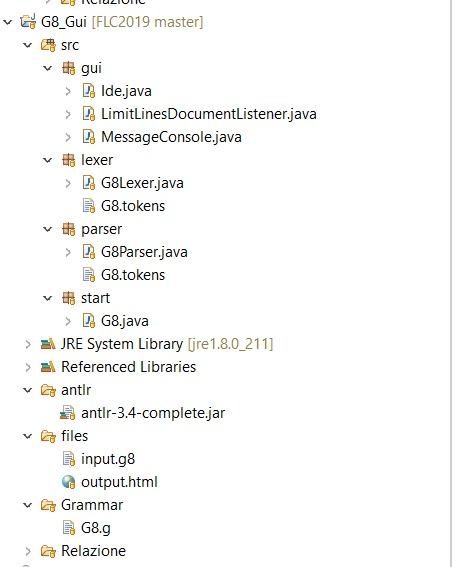
\includegraphics[scale=2.5]{progetto.jpg} 
\end{center}

\newpage

\subsection{Editor}

We have developed a dedicated editor for assisted writing of the G8 language.
The "Save" button allows you to save the code written in the TextArea.
With "Load" the user can load the contents of a text file in the textArea.
The "Draw" button allows you to draw figures written with G8.
Then there are buttons on the right that assist the user by entering an example of the figure indicated by the button.
The "EXAMPLE" button inserts an example for all the figures.\\
\begin{center}
\includegraphics[scale=2.5]{editor.jpg} 
\end{center}

\newpage

\section{G8 structure}

First the user must initialize the project and enter the title of his work, the width of the drawing area and the height of the same. The syntax is as follows:
\vspace{1\baselineskip}
\begin{verbatim}
TITLE titleText DRAWSPACE WIDTH widthFloat DRAWSPACE HEIGTH heigthFloat
\end{verbatim}
\vspace{1\baselineskip}
The user can draw a figure between: line, triangle, rectangle, curve, circle and ellipse. Every figure has mandatory values for the measurements that will go from (0, 0), top left corner of the screen, to the maximum value chosen for the drawing area and optional values, related to color, thickness, filling, rotation, etc. It is also possible to name the figure as desired: in case a name is not given it will be set to the default value "no name".
\vspace{1\baselineskip}
\begin{itemize}
\item \textbf{line}: mandatory entry of departure and arrival coordinates is required. The user can also insert, optionally, the color and thickness of the line: in case they are not entered manually, the default values (black color, thickness 1) will be used. The syntax is as follows:
\vspace{1\baselineskip}
\begin{verbatim}
LINE: (NAME nameText) XSTART startAbscissaFloat YSTART startOrdinateFloat XEND endAbscissaFloat 
YEND endOrdinateFloat (COLOR colorRGB WIDTH thicknessFloat)
\end{verbatim}
\vspace{1\baselineskip}
\item \textbf{triangle}: mandatory entry of the coordinates of the three vertices is required. The user can also insert, optionally, the color of the border, the thickness of the border and the filling of the figure: in case they are not entered manually, the default values (black border color, thickness 1, transparent fill color) will be used. The syntax is as follows:
\vspace{1\baselineskip}
\begin{verbatim}
TRIANGLE: (NAME nameText) XA OneAbscissaFloat YA oneOrdinateFloat XB twoAbscissaFloat YB 
twoOrdinateFloat XC threeAbscissaFloat YC threeOrdinateFloat (COLOR
colorBorderRGB WIDTH thicknessFloat COLORBODY colorBodyRGB)
\end{verbatim}
\vspace{1\baselineskip}
\item \textbf{rectangle}: it is mandatory to enter the coordinates of the two opposite vertices. The user can also insert, optionally, the color of the border, the thickness of the border and the filling of the figure: in case they are not entered manually, the default values (black border color, thickness 1, transparent fill color) will be used. The syntax is as follows:
\vspace{1\baselineskip}
\begin{verbatim}
RECT: (NAME nameText) XSTART oneAbscissaFloat YSTART oneOrdinateFloat XEND twoAbscissaFloat YEND 
twoOrdinateFloat (COLOR colorBorderRGB WIDTH thicknessFloat COLORBODY colorBodyRGB)
\end{verbatim}
\vspace{1\baselineskip}
\item \textbf{curve}: 
it is mandatory to enter the coordinates of the starting point, the arrival point and the curve point. The user can also insert, optionally, the color of the border, the thickness of the border and the filling of the figure: in case they are not entered manually, the default values (black border color, thickness 1, transparent fill color) will be used. The syntax is as follows:
\vspace{1\baselineskip}
\begin{verbatim}
CURV: (NAME nameText) XSTART OneAbscissaFloat YSTART oneOrdinateFloat XMIDDLE
curvatureAbscissaFloat YMIDDLE curvatureOrdinateFloat XEND twoAbscissaFloat YEND 
twoOrdinateFloat (COLOR colorBorderRGB WIDTH thicknessFloat 
COLORBODY colorBodyRGB)
\end{verbatim}
\vspace{1\baselineskip}
\item \textbf{circle}: 
it is mandatory to insert the center and radius coordinates. The user can also insert, optionally, the color of the border, the thickness of the border and the filling of the figure: in case they are not entered manually, the default values (black border color, thickness 1, transparent fill color) will be used. Another optional element to enter is relative to the starting and ending angle: it is in fact possible to create partial circumferences or semicircles, inserting limits for the angle to be represented; if they are not entered manually, the default values (0 as start angle and 360 as end angle) will be used, developing the entire circumference. The syntax is as follows:
\vspace{1\baselineskip}
\begin{verbatim}
CIRC: (NAME nameText) XCENTER centerAbscissaFloat YCENTER centerOrdinateFloat RADIUS radiusFloat
STARTANGLE angleFloat ENDANGLE angleFloat COLOR colorRGB  WIDTH thicknessFloat 
COLORBODY colorBodyRGB)
\end{verbatim}
\vspace{1\baselineskip}
\item \textbf{ellipse}: it is mandatory to enter the coordinates of the center, of the semi-major axis and of the semi-minor axis. The user can also insert, optionally, the color of the border, the thickness of the border and the filling of the figure: in case they are not entered manually, the default values (black border color, thickness 1, transparent fill color) will be used. Another optional element to be inserted is relative to the starting and ending angle: it is in fact possible to create partial or semi-circumferential circles, inserting limits for the angle to be represented; if they are not entered manually, the default values (0 as start angle and 360 as end angle) will be used, realizing the entire circumference. It is also possible to assign a value of rotation of the ellipse around its origin, by rotating a positive or negative value of degrees; if it is not entered manually the default value will be used which does not assign any rotation (0 as angle of rotation). The syntax is as follows:
\vspace{1\baselineskip}
\begin{verbatim}
ELLIPS: (NAME nameText) XCENTER centerAbscissaFloat YCENTER centerOrdinateFloat 
SEMIN minAxisFloat SEMAX maxAxisFloat (STARTANGLE angleFloat ENDANGLE angleFloat ROTATION
rotationDegree COLOR colorBorderRGB WIDTH thicknessFloat 
COLORBODY colorBodyFloat)
\end{verbatim}
\vspace{1\baselineskip}
\end{itemize}
At the end of the code the user must write "END" :
\begin{verbatim}
END
\end{verbatim}

\newpage

\section{A first basic example}

The following example clearly shows the potential of the G8 language; in fact, only five lines of code were needed to draw 3 figures.
The resulting figure represents the symbol of the "Deathly Hallows", taken from the Harry Potter saga by J.K. Rowling.

\subsection{Canvas-HTML5 Version}
\begin{verbatim}
TITLE prova DRAWSPACE WIDTH 1000 DRAWSPACE HEIGTH 1000
TRIANGLE: NAME cloak XA 457 YA 252 XB 215 YB 608 XC 699 YC 608 WIDTH 3
CIRC: NAME stone XCENTER 457 YCENTER 480 RADIUS 128 WIDTH 3
LINE: NAME wand XSTART 457 YSTART 608 XEND 457 YEND 252 WIDTH 3
END
\end{verbatim}

\subsection{G8 Version}
\begin{verbatim}
<!doctype html>
<html>
<head>
<title> prova </title>
<style> canvas {border: 1px #000 dotted;} </style>
<script>
window.onload = function () {

	var canvas = document.getElementById('prova');
	var context = canvas.getContext('2d'); 

	//cloak
	context.beginPath();
	context.lineWidth = 3.0;
	context.strokeStyle = '#000000';
	context.moveTo(457.0, 252.0);
	context.lineTo(215.0, 608.0);
	context.lineTo(699.0, 608.0);
	context.lineTo(457.0, 252.0);
	context.stroke();
	context.closePath();

	//stone
	context.beginPath();
	var centerX = 457.0;
	var centerY = 480.0;
	var radius = 128.0;
	var startAngle = 0.0* Math.PI/180;
	var endAngle = 360.0* Math.PI/180;
	context.arc (centerX, centerY, radius, startAngle, endAngle);
	context.lineWidth = 3.0;
	context.strokeStyle= '#000000';
	context.stroke();
	context.closePath();

	//wand
	context.beginPath();
	context.lineWidth = 3.0;
	context.strokeStyle = '#000000';
	context.moveTo( 457.0, 608.0);
	context.lineTo( 457.0, 252.0);
	context.stroke();
	context.closePath();

}
</script>
</head>
<body>
<canvas id='prova' width='1000.0' height='1000.0'></canvas>
</body>
</html>

\end{verbatim}

\subsection{Result}
\begin{center}
 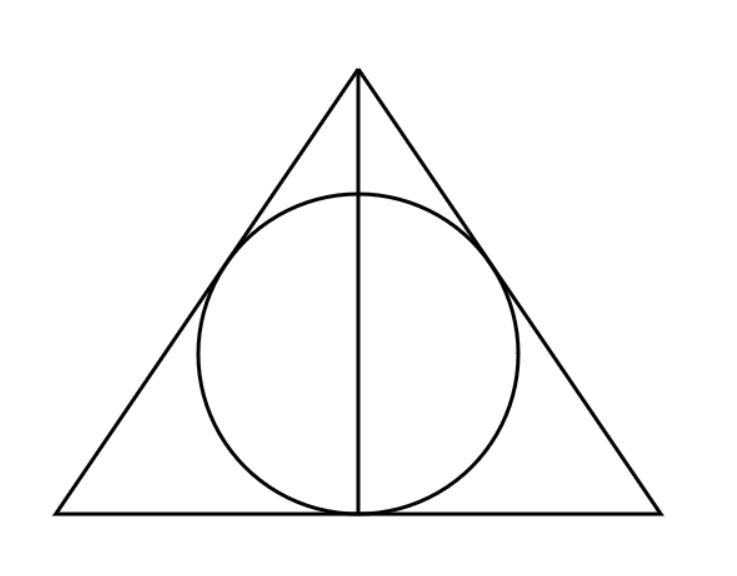
\includegraphics[scale=1.0]{hp.JPG}
 \end{center} 



\newpage


\section{A more complex example}

As a more complete practical example we have created a representation of the face of Mickey Mouse, a character created in 1928 by Walter Elias Disney and today a symbol of the multinational The Walt Disney Company.
\\
\\
Below we will show the code needed to create the logo in Canvas HTML5, then the code in our G8 language and finally the graphic result.

\subsection{Canvas-HTML5 Version}
\begin{verbatim}
<!doctype html>
<html>
<head>
<title> Topolino </title>
<style> canvas {border: 1px #000 dotted;} </style>
<script>
window.onload = function () {

	var canvas = document.getElementById('Topolino');
	var context = canvas.getContext('2d'); 

	//CirconferenzaViso
	context.beginPath();
	var centerX = 850.0;
	var centerY = 550.0;
	var radius = 300.0;
	var startAngle = 0.0* Math.PI/180;
	var endAngle = 360.0* Math.PI/180;
	context.arc (centerX, centerY, radius, startAngle, endAngle);
	context.lineWidth = 0.0;
	context.strokeStyle= '#000000';
	context.stroke();
	context.fillStyle= '#000000';
	context.fill();
	context.closePath();

	//EllisseOrecchioSinistro
	context.beginPath();
	var centerX = 600.0;
	var centerY = 210.0;
	var radiusMax = 170.0;
	var radiusMin= 130.0;
	var rotation= -45.0*Math.PI/180;
	var startAngle=0.0*Math.PI/180;
	var endAngle=360.0*Math.PI/180;
	context.ellipse(centerX, centerY, radiusMax, radiusMin, rotation, startAngle, endAngle);
	context.lineWidth = 0.0;
	context.strokeStyle= '#000000';
	context.stroke();
	context.fillStyle= '#000000';
	context.fill();
	context.closePath();

	//EllisseOrecchioDestro
	context.beginPath();
	var centerX = 1100.0;
	var centerY = 210.0;
	var radiusMax = 170.0;
	var radiusMin= 130.0;
	var rotation= 45.0*Math.PI/180;
	var startAngle=0.0*Math.PI/180;
	var endAngle=360.0*Math.PI/180;
	context.ellipse(centerX, centerY, radiusMax, radiusMin, rotation, startAngle, endAngle);
	context.lineWidth = 0.0;
	context.strokeStyle= '#000000';
	context.stroke();
	context.fillStyle= '#000000';
	context.fill();
	context.closePath();

	//EllisseParteAltaSinistraViso
	context.beginPath();
	var centerX = 750.0;
	var centerY = 450.0;
	var radiusMax = 120.0;
	var radiusMin= 170.0;
	var rotation= 0.0*Math.PI/180;
	var startAngle=0.0*Math.PI/180;
	var endAngle=360.0*Math.PI/180;
	context.ellipse(centerX, centerY, radiusMax, radiusMin, rotation, startAngle, endAngle);
	context.lineWidth = 0.0;
	context.strokeStyle= '#FFFFFF';
	context.stroke();
	context.fillStyle= '#FFFFFF';
	context.fill();
	context.closePath();

	//EllisseParteAltaDestraViso
	context.beginPath();
	var centerX = 950.0;
	var centerY = 450.0;
	var radiusMax = 120.0;
	var radiusMin= 170.0;
	var rotation= 0.0*Math.PI/180;
	var startAngle=0.0*Math.PI/180;
	var endAngle=360.0*Math.PI/180;
	context.ellipse(centerX, centerY, radiusMax, radiusMin, rotation, startAngle, endAngle);
	context.lineWidth = 0.0;
	context.strokeStyle= '#FFFFFF';
	context.stroke();
	context.fillStyle= '#FFFFFF';
	context.fill();
	context.closePath();

	//CerchioInferioreCoperturaNero
	context.beginPath();
	var centerX = 850.0;
	var centerY = 550.0;
	var radius = 299.0;
	var startAngle = 16.2* Math.PI/180;
	var endAngle = 163.8* Math.PI/180;
	context.arc (centerX, centerY, radius, startAngle, endAngle);
	context.lineWidth = 0.0;
	context.strokeStyle= '#FFFFFF';
	context.stroke();
	context.fillStyle= '#FFFFFF';
	context.fill();
	context.closePath();

	//CurvaGuanciaSinistra
	context.beginPath();
	context.lineWidth = 0.0;
	context.strokeStyle = '#FFFFFF';
	context.moveTo( 566.0, 642.0);
	context.quadraticCurveTo( 580.0, 560.0, 672.0, 580.0);
	context.stroke();
	context.fillStyle= '#FFFFFF';
	context.fill();
	context.closePath();

	//CurvaGuanciaDestra
	context.beginPath();
	context.lineWidth = 0.0;
	context.strokeStyle = '#FFFFFF';
	context.moveTo( 1028.0, 580.0);
	context.quadraticCurveTo( 1103.0, 560.0, 1136.0, 642.0);
	context.stroke();
	context.fillStyle= '#FFFFFF';
	context.fill();
	context.closePath();

	//TriangoloCoperturaNeroCentrale
	context.beginPath();
	context.lineWidth = 0.0;
	context.strokeStyle = '#FFFFFF';
	context.moveTo(566.0, 641.0);
	context.lineTo(1134.0, 641.0);
	context.lineTo(850.0, 476.0);
	context.lineTo(566.0, 641.0);
	context.stroke();
	context.fillStyle= '#FFFFFF';
	context.fill();
	context.closePath();

	//EllisseOcchioSinistro
	context.beginPath();
	var centerX = 788.0;
	var centerY = 450.0;
	var radiusMax = 40.0;
	var radiusMin= 100.0;
	var rotation= 0.0*Math.PI/180;
	var startAngle=0.0*Math.PI/180;
	var endAngle=360.0*Math.PI/180;
	context.ellipse(centerX, centerY, radiusMax, radiusMin, rotation, startAngle, endAngle);
	context.lineWidth = 3.0;
	context.strokeStyle= '#000000';
	context.stroke();
	context.closePath();

	//EllisseOcchioDestro
	context.beginPath();
	var centerX = 912.0;
	var centerY = 450.0;
	var radiusMax = 40.0;
	var radiusMin= 100.0;
	var rotation= 0.0*Math.PI/180;
	var startAngle=0.0*Math.PI/180;
	var endAngle=360.0*Math.PI/180;
	context.ellipse(centerX, centerY, radiusMax, radiusMin, rotation, startAngle, endAngle);
	context.lineWidth = 3.0;
	context.strokeStyle= '#000000';
	context.stroke();
	context.closePath();

	//EllissePupillaSinistra
	context.beginPath();
	var centerX = 810.0;
	var centerY = 480.0;
	var radiusMax = 15.0;
	var radiusMin= 40.0;
	var rotation= 0.0*Math.PI/180;
	var startAngle=0.0*Math.PI/180;
	var endAngle=360.0*Math.PI/180;
	context.ellipse(centerX, centerY, radiusMax, radiusMin, rotation, startAngle, endAngle);
	context.lineWidth = 0.0;
	context.strokeStyle= '#000000';
	context.stroke();
	context.fillStyle= '#000000';
	context.fill();
	context.closePath();

	//EllissePupillaDestra
	context.beginPath();
	var centerX = 890.0;
	var centerY = 480.0;
	var radiusMax = 15.0;
	var radiusMin= 40.0;
	var rotation= 0.0*Math.PI/180;
	var startAngle=0.0*Math.PI/180;
	var endAngle=360.0*Math.PI/180;
	context.ellipse(centerX, centerY, radiusMax, radiusMin, rotation, startAngle, endAngle);
	context.lineWidth = 0.0;
	context.strokeStyle= '#000000';
	context.stroke();
	context.fillStyle= '#000000';
	context.fill();
	context.closePath();

	//CurvaSottoOcchi
	context.beginPath();
	context.lineWidth = 6.0;
	context.strokeStyle = '#000000';
	context.moveTo( 740.0, 552.0);
	context.quadraticCurveTo( 850.0, 470.0, 960.0, 552.0);
	context.stroke();
	context.fillStyle= '#FFFFFF';
	context.fill();
	context.closePath();

	//CirconferenzaCopriCurvaOcchiSinistra
	context.beginPath();
	var centerX = 740.0;
	var centerY = 552.0;
	var radius = 3.0;
	var startAngle = 0.0* Math.PI/180;
	var endAngle = 360.0* Math.PI/180;
	context.arc (centerX, centerY, radius, startAngle, endAngle);
	context.lineWidth = 0.0;
	context.strokeStyle= '#FFFFFF';
	context.stroke();
	context.fillStyle= '#FFFFFF';
	context.fill();
	context.closePath();

	//CirconferenzaCopriCurvaOcchiDestra
	context.beginPath();
	var centerX = 960.0;
	var centerY = 552.0;
	var radius = 3.0;
	var startAngle = 0.0* Math.PI/180;
	var endAngle = 360.0* Math.PI/180;
	context.arc (centerX, centerY, radius, startAngle, endAngle);
	context.lineWidth = 0.0;
	context.strokeStyle= '#FFFFFF';
	context.stroke();
	context.fillStyle= '#FFFFFF';
	context.fill();
	context.closePath();

	//CurvaMento
	context.beginPath();
	context.lineWidth = 2.0;
	context.strokeStyle = '#000000';
	context.moveTo( 700.0, 750.0);
	context.quadraticCurveTo( 850.0, 980.0, 1000.0, 750.0);
	context.stroke();
	context.fillStyle= '#FFFFFF';
	context.fill();
	context.closePath();

	//CurvaLabbroInferiore
	context.beginPath();
	context.lineWidth = 4.0;
	context.strokeStyle = '#000000';
	context.moveTo( 700.0, 696.0);
	context.quadraticCurveTo( 850.0, 990.0, 1000.0, 696.0);
	context.stroke();
	context.fillStyle= '#000000';
	context.fill();
	context.closePath();

	//CurvaLabbroSuperiore
	context.beginPath();
	context.lineWidth = 4.0;
	context.strokeStyle = '#000000';
	context.moveTo( 620.0, 635.0);
	context.quadraticCurveTo( 850.0, 850.0, 1080.0, 635.0);
	context.stroke();
	context.fillStyle= '#FFFFFF';
	context.fill();
	context.closePath();

	//CurvaLabbroSinistro
	context.beginPath();
	context.lineWidth = 3.0;
	context.strokeStyle = '#000000';
	context.moveTo( 598.0, 658.0);
	context.quadraticCurveTo( 625.0, 625.0, 653.0, 623.0);
	context.stroke();
	context.closePath();

	//CurvaLabbroDestro
	context.beginPath();
	context.lineWidth = 3.0;
	context.strokeStyle = '#000000';
	context.moveTo( 1102.0, 658.0);
	context.quadraticCurveTo( 1075.0, 625.0, 1047.0, 623.0);
	context.stroke();
	context.closePath();

	//EllisseNaso
	context.beginPath();
	var centerX = 850.0;
	var centerY = 600.0;
	var radiusMax = 65.0;
	var radiusMin= 50.0;
	var rotation= 0.0*Math.PI/180;
	var startAngle=0.0*Math.PI/180;
	var endAngle=360.0*Math.PI/180;
	context.ellipse(centerX, centerY, radiusMax, radiusMin, rotation, startAngle, endAngle);
	context.lineWidth = 0.0;
	context.strokeStyle= '#000000';
	context.stroke();
	context.fillStyle= '#000000';
	context.fill();
	context.closePath();

	//CerchioCopriMentoSinistro
	context.beginPath();
	var centerX = 700.0;
	var centerY = 773.0;
	var radius = 22.0;
	var startAngle = 0.0* Math.PI/180;
	var endAngle = 360.0* Math.PI/180;
	context.arc (centerX, centerY, radius, startAngle, endAngle);
	context.lineWidth = 0.0;
	context.strokeStyle= '#FFFFFF';
	context.stroke();
	context.fillStyle= '#FFFFFF';
	context.fill();
	context.closePath();

	//CerchioCopriMentoDestro
	context.beginPath();
	var centerX = 1000.0;
	var centerY = 773.0;
	var radius = 22.0;
	var startAngle = 0.0* Math.PI/180;
	var endAngle = 360.0* Math.PI/180;
	context.arc (centerX, centerY, radius, startAngle, endAngle);
	context.lineWidth = 0.0;
	context.strokeStyle= '#FFFFFF';
	context.stroke();
	context.fillStyle= '#FFFFFF';
	context.fill();
	context.closePath();

	//TerminaCirconferenzaViso
	context.beginPath();
	context.lineWidth = 0.0;
	context.strokeStyle = '#000000';
	context.moveTo( 1137.0, 642.0);
	context.quadraticCurveTo( 1137.0, 642.0, 1137.0, 641.0);
	context.stroke();
	context.closePath();

	//CerchioCopriTerminaCirconferenzaViso
	context.beginPath();
	var centerX = 1139.0;
	var centerY = 642.0;
	var radius = 1.0;
	var startAngle = 0.0* Math.PI/180;
	var endAngle = 360.0* Math.PI/180;
	context.arc (centerX, centerY, radius, startAngle, endAngle);
	context.lineWidth = 0.0;
	context.strokeStyle= '#FFFFFF';
	context.stroke();
	context.fillStyle= '#FFFFFF';
	context.fill();
	context.closePath();

	//EllisseLinguaSinistra
	context.beginPath();
	var centerX = 829.0;
	var centerY = 816.0;
	var radiusMax = 46.0;
	var radiusMin= 25.0;
	var rotation= 18.0*Math.PI/180;
	var startAngle=0.0*Math.PI/180;
	var endAngle=360.0*Math.PI/180;
	context.ellipse(centerX, centerY, radiusMax, radiusMin, rotation, startAngle, endAngle);
	context.lineWidth = 0.0;
	context.strokeStyle= '#FF0000';
	context.stroke();
	context.fillStyle= '#FF0000';
	context.fill();
	context.closePath();

	//EllisseLinguaDestra
	context.beginPath();
	var centerX = 867.0;
	var centerY = 817.0;
	var radiusMax = 46.0;
	var radiusMin= 25.0;
	var rotation= -18.0*Math.PI/180;
	var startAngle=0.0*Math.PI/180;
	var endAngle=360.0*Math.PI/180;
	context.ellipse(centerX, centerY, radiusMax, radiusMin, rotation, startAngle, endAngle);
	context.lineWidth = 0.0;
	context.strokeStyle= '#FF0000';
	context.stroke();
	context.fillStyle= '#FF0000';
	context.fill();
	context.closePath();

	//LineaLingua
	context.beginPath();
	context.lineWidth = 2.0;
	context.strokeStyle = '#000000';
	context.moveTo( 842.0, 792.0);
	context.quadraticCurveTo( 870.0, 803.0, 870.0, 815.0);
	context.stroke();
	context.closePath();

}
</script>
</head>
<body>
<canvas id='Topolino' width='1700.0' height='900.0'></canvas>
</body>
</html>
\end{verbatim}

\newpage

\subsection{G8 version}
\begin{verbatim}
TITLE Topolino DRAWSPACE WIDTH 1700 DRAWSPACE HEIGTH 900
CIRC: NAME CirconferenzaViso XCENTER 850 YCENTER 550 RADIUS 300 COLORBODY #000000
ELLIPS: NAME EllisseOrecchioSinistro XCENTER 600 YCENTER 210 SEMIN 130 SEMAX 170 ROTATION -45
COLORBODY #000000
ELLIPS: NAME EllisseOrecchioDestro XCENTER 1100 YCENTER 210 SEMIN 130 SEMAX 170 ROTATION +45
COLORBODY #000000
ELLIPS: NAME EllisseParteAltaSinistraViso XCENTER 750 YCENTER 450 SEMIN 170 SEMAX 120 COLOR
#FFFFFF COLORBODY #FFFFFF
ELLIPS: NAME EllisseParteAltaDestraViso XCENTER 950 YCENTER 450 SEMIN 170 SEMAX 120 COLOR #FFFFFF
COLORBODY #FFFFFF
CIRC: NAME CerchioInferioreCoperturaNero XCENTER 850 YCENTER 550 RADIUS 299 STARTANGLE 16.2
ENDANGLE 163.8 COLOR #FFFFFF COLORBODY #FFFFFF
CURV: NAME CurvaGuanciaSinistra XSTART 566 YSTART 642 XMIDDLE 580 YMIDDLE 560 XEND 672 YEND 580
COLOR #FFFFFF COLORBODY #FFFFFF
CURV: NAME CurvaGuanciaDestra XSTART 1028 YSTART 580 XMIDDLE 1103 YMIDDLE 560 XEND 1136 YEND 642
COLOR #FFFFFF COLORBODY #FFFFFF
TRIANGLE: NAME TriangoloCoperturaNeroCentrale XA 566 YA 641 XB 1134 YB 641 XC 850 YC 476 COLOR
#FFFFFF COLORBODY #FFFFFF
ELLIPS: NAME EllisseOcchioSinistro XCENTER 788 YCENTER 450 SEMIN 100 SEMAX 40 WIDTH 3
ELLIPS: NAME EllisseOcchioDestro XCENTER 912 YCENTER 450 SEMIN 100 SEMAX 40 WIDTH 3
ELLIPS: NAME EllissePupillaSinistra XCENTER 810 YCENTER 480 SEMIN 40 SEMAX 15 COLORBODY #000000
ELLIPS: NAME EllissePupillaDestra XCENTER 890 YCENTER 480 SEMIN 40 SEMAX 15 COLORBODY #000000
CURV: NAME CurvaSottoOcchi XSTART 740 YSTART 552 XMIDDLE 850 YMIDDLE 470 XEND 960 YEND 552 WIDTH
6 COLORBODY #FFFFFF
CIRC: NAME CirconferenzaCopriCurvaOcchiSinistra XCENTER 740 YCENTER 552 RADIUS 3 COLOR #FFFFFF
COLORBODY #FFFFFF
CIRC: NAME CirconferenzaCopriCurvaOcchiDestra XCENTER 960 YCENTER 552 RADIUS 3 COLOR #FFFFFF
COLORBODY #FFFFFF
CURV: NAME CurvaMento XSTART 700 YSTART 750 XMIDDLE 850 YMIDDLE 980 XEND 1000 YEND 750 WIDTH 2
COLORBODY #FFFFFF
CURV: NAME CurvaLabbroInferiore XSTART 700 YSTART 696 XMIDDLE 850 YMIDDLE 990 XEND 1000 YEND 696
WIDTH 4 COLORBODY #000000
CURV: NAME CurvaLabbroSuperiore XSTART 620 YSTART 635 XMIDDLE 850 YMIDDLE 850 XEND 1080 YEND 635
WIDTH 4 COLORBODY #FFFFFF
CURV: NAME CurvaLabbroSinistro XSTART 598 YSTART 658 XMIDDLE 625 YMIDDLE 625 XEND 653 YEND 623
WIDTH 3
CURV: NAME CurvaLabbroDestro XSTART 1102 YSTART 658 XMIDDLE 1075 YMIDDLE 625 XEND 1047 YEND 623
WIDTH 3
ELLIPS: NAME EllisseNaso XCENTER 850 YCENTER 600 SEMIN 50 SEMAX 65 COLORBODY #000000
CIRC: NAME CerchioCopriMentoSinistro XCENTER 700 YCENTER 773 RADIUS 22 COLOR #FFFFFF COLORBODY
#FFFFFF
CIRC: NAME CerchioCopriMentoDestro XCENTER 1000 YCENTER 773 RADIUS 22 COLOR #FFFFFF COLORBODY
#FFFFFF
CURV: NAME TerminaCirconferenzaViso XSTART 1137 YSTART 642 XMIDDLE 1137 YMIDDLE 642 XEND 1137
YEND 641
CIRC: NAME CerchioCopriTerminaCirconferenzaViso XCENTER 1139 YCENTER 642 RADIUS 1 COLOR #FFFFFF
COLORBODY #FFFFFF
ELLIPS: NAME EllisseLinguaSinistra XCENTER 829 YCENTER 816 SEMIN 25 SEMAX 46 ROTATION +18 COLOR
#FF0000 COLORBODY #FF0000
ELLIPS: NAME EllisseLinguaDestra XCENTER 867 YCENTER 817 SEMIN 25 SEMAX 46 ROTATION -18 COLOR
#FF0000 COLORBODY #FF0000
CURV: NAME LineaLingua XSTART 842 YSTART 792 XMIDDLE 870 YMIDDLE 803 XEND 870 YEND 815 WIDTH 2
END
\end{verbatim}

\newpage

\subsection{Result}

\includegraphics[scale=0.76]{Topolino.JPG} 

\newpage

\section{Conclusions}


The tool created allows you to generate HTML5-Canvas code based on some predefined instructions and requires you to insert fewer characters and lines of code.
G8 can be improved by adding other drawable shapes.
The project had the purpose of making the drawing of canvas figures simpler and faster and the objective was achieved.

\vspace{2\baselineskip}

\section{Sitography}

\begin{enumerate}
\item ANTLRWorks -  \href{https://www.antlr3.org/works/}{$https://www.antlr3.org/works/$} 
\item ANTLR - \href{http://www.antlr.org/}{$http://www.antlr.org/$}
\item Grammar - \href{https://github.com/Stefanoga/G8_Gui/blob/master/G8/Grammar/G8.g}{$https://github.com/Stefanoga/G8_Gui/blob/master/G8/Grammar/G8.g$}
\label{grammar}
\item G8 Project - \href{https://github.com/Stefanoga/G8_Eclipse}{$https://github.com/Stefanoga/G8_Eclipse$}
\item G8 Project with GUI Editor - \href{https://github.com/Stefanoga/G8_Gui}{$https://github.com/Stefanoga/G8_Gui$}
\end{enumerate}

\end{document}